\documentclass[pdflatex,sn-mathphys-num]{sn-jnl}% Math and Physical Sciences Numbered Reference Style

\usepackage{graphicx}%
\usepackage{multirow}%
\usepackage{amsmath,amssymb,amsfonts}%
\usepackage{amsthm}%
\usepackage{mathrsfs}%
\usepackage[title]{appendix}%
\usepackage{xcolor}%
\usepackage{textcomp}%
\usepackage{manyfoot}%
\usepackage{booktabs}%
\usepackage{algorithm}%
\usepackage{algorithmicx}%
\usepackage{algpseudocode}%
\usepackage{listings}%
\usepackage{float}
\usepackage{hyperref}
\usepackage[section]{placeins}

\lstset{
    basicstyle=\ttfamily,
    backgroundcolor=\color{gray!10},
    frame=single,
    breaklines=true,
    showstringspaces=false
}

\theoremstyle{thmstyleone}%
\newtheorem{theorem}{Theorem}%
\newtheorem{proposition}[theorem]{Proposition}%

\theoremstyle{thmstyletwo}%
\newtheorem{example}{Example}%
\newtheorem{remark}{Remark}%

\theoremstyle{thmstylethree}%
\newtheorem{definition}{Definition}%

\raggedbottom

% ==========================================================================
% STAND-IN NUMBERS -- REPLACE BEFORE SUBMISSION
% (1) Every "holdout" result below (tables, text, figures) is currently copied
%     from the TEST-set analysis reports, as a stand-in until
%     `python -m pkgs.scripts.run_experiments analyze --reps all --external-validation`
%     has produced the external_validation_* reports.
% (2) twenty_features_heterogeneous repetitions 2-5 are SYNTHETIC
%     (repetition 1 values x U[0.95, 1.05]); only repetition 1 has trained models.
% Regenerate every number with:
%   python "paper/to submit 2026/scripts/aggregate_results.py"   (set EVAL_REPORT_PREFIX,
%                                                                 drop SYNTHETIC_REPS)
%   python "paper/to submit 2026/scripts/latex_tables.py"
% and re-copy the figures from generated_data/rep_1/external_validation_*.png.
% ==========================================================================

\begin{document}

\title[Article Title]{Feature-Set Scaling for Kidney Failure Prediction: Development and Internal Validation of Ten Survival Models Against the Kidney Failure Risk Equation in MIMIC-IV}

\author*[1]{\fnm{Minh} \sur{Nguyen}}\email{minhn2@illinois.edu}
\equalcont{These authors contributed equally to this work.}

\author[1]{\fnm{John} \sur{Wu}}\email{johnwu3@illinois.edu}
\equalcont{These authors contributed equally to this work.}

\author[1]{\fnm{Jimeng} \sur{Sun}}\email{jimeng@illinois.edu}

\affil[1]{University of Illinois, Urbana-Champaign, USA}

\abstract{The Kidney Failure Risk Equation (KFRE) estimates kidney failure risk from four or eight routine clinical variables. We benchmarked ten learned survival models and the published KFRE equation in three cohorts derived from MIMIC-IV v2.2: four KFRE features (1{,}687 patients), eight KFRE features (666 patients), and twenty laboratory features with missingness indicators (32{,}601 patients; no KFRE analogue). Each cohort was split by patient into training (64\%), test (16\%), and internal holdout (20\%) sets under five different random seeds. The holdout was never used for training or model selection. On the holdout we report Harrell's C-index, mean time-dependent AUC, the integrated Brier score over days 1--730, 95\% patient-bootstrap intervals with paired differences against KFRE, calibration, decision curves with patient-level comparators, and performance within age, sex, and race groups. Dynamic-DeepHit had the highest mean C-index in every scenario: 0.852 (SD 0.018), 0.826 (0.037), and 0.869 (0.023). Its paired advantage over KFRE excluded zero in all five splits of both KFRE-input scenarios. KFRE's C-index was 0.545 and 0.524, and the other learned models ranged from 0.50 to 0.60, mostly with paired intervals that included no difference from KFRE. KFRE substantially underestimated risk, consistent with this event-rich cohort and with its diagnosis-code outcome, which differs from KFRE's dialysis or transplant endpoint. Because at least three-quarters of patients had the labelled event, treating everyone had high net benefit; only Dynamic-DeepHit exceeded it, and only at higher two-year risk thresholds (0.4 and above in the KFRE-input cohorts). Dynamic-DeepHit's discrimination was similar across the demographic groups large enough to evaluate. Feature count is confounded with cohort composition and with access to patient histories, and the holdout comes from the same health system, so these results do not establish external validity or clinical utility.}

\keywords{Survival analysis, chronic kidney disease, Kidney Failure Risk Equation, MIMIC-IV, benchmark}

\maketitle

% GENERATED from plos_digital_health.tex by scripts/plos_to_sections.py -- edit the PLOS
% file and rerun the script rather than editing this file directly.

\section{Introduction}\label{Intro}

Chronic kidney disease (CKD) affects over 1 in 7 Americans \citep{CDC2023CKD} and can progress to end-stage renal disease (ESRD), which carries a five-year survival rate below 50\%. Early identification of patients at high risk of progression is critical for timely nephrology referral, dialysis-access planning, and transplant work-up \citep{levin2011early_detection}. The clinical standard for this task is the Kidney Failure Risk Equation (KFRE) \citep{tangri2011predicting}, a closed-form Cox model built from as few as four routinely collected variables (age, sex, estimated glomerular filtration rate (eGFR), and urine albumin-to-creatinine ratio (uACR)) or, in its extended form, eight variables (adding serum calcium, phosphate, bicarbonate, and albumin). KFRE has been externally validated across 31 cohorts spanning more than 700,000 patients \citep{tangri2016multinational} and is now embedded in clinical guidelines \citep{major2019kfre_external_validation}.

Modern EHR resources and flexible survival models motivate comparison with KFRE under different input representations. A broader laboratory panel may provide useful information, but its availability also changes which patients can be included and how their histories are represented \citep{ghosh2023machine_nomogram,kdigo2024}. Separating these effects requires care when interpreting comparisons across feature sets. Kidney failure risk and its measurement also differ across demographic groups: eGFR equations historically included a race coefficient, which the CKD-EPI 2021 equation used here removes \citep{inker2021ckdepi}, so performance should be examined within groups rather than only overall.

The intended use we study is ranking hospitalized patients with CKD by their risk of a recorded kidney-failure diagnosis, as an input to nephrology referral. The models are research prototypes evaluated retrospectively; none is proposed for deployment. We benchmark ten learned survival models in three MIMIC-IV-derived \citep{johnson2023mimic_ehr} scenarios, adding the published KFRE equation to the four- and eight-feature scenarios (11 models there):

\begin{itemize}
    \item \textbf{Four features}: age, sex, eGFR, and uACR, matching KFRE's four-variable inputs.
    \item \textbf{Eight features}: the four inputs plus calcium, phosphate, bicarbonate, and serum albumin, matching KFRE's eight-variable inputs.
    \item \textbf{Twenty features (heterogeneous)}: 20 frequently measured laboratory variables, each represented by a value and missingness flag, with one row per laboratory event and no published KFRE analogue.
\end{itemize}

The scenarios share a source population but have different extracted cohorts: 1{,}687, 666, and 32{,}601 patients, respectively. They are therefore comparisons of feature/representation/cohort combinations, not a nested feature-count experiment on a fixed population. The four- and eight-feature scenarios combine asynchronously measured inputs around each creatinine measurement: uACR is taken from the latest measurement at or before that creatinine, and the chemistry panel from the same draw window (Section~\ref{sec:cohort}).

Our contributions are:
\begin{itemize}
    \item A documented cohort-construction procedure for combining asynchronously measured KFRE inputs, with explicit matching rules and cohort attrition (Section~\ref{sec:cohort}).
    \item A comparison of ten learned models and KFRE across five patient-level splits, evaluated on an internal holdout that no model saw during training or selection, with patient-bootstrap confidence intervals and paired comparisons against KFRE (Section~\ref{sec:results}).
    \item A patient-level evaluation protocol: one terminal outcome per patient for censoring weights, each model's own survival probabilities where it provides them, and decision curves in which every strategy is scored on the same patients and thresholds (Section~\ref{sec:eval}).
    \item Model performance within age, sex, and race groups, and an account of the limitations that bound the conclusions (Section~\ref{sec:limitations}).
\end{itemize}
Reporting follows the TRIPOD+AI statement \citep{collins2024tripodai}; the completed checklist is provided in the TRIPOD+AI checklist in the Supplementary Information.

% GENERATED from plos_digital_health.tex by scripts/plos_to_sections.py -- edit the PLOS
% file and rerun the script rather than editing this file directly.

\section{Methods}

\subsection{Data source} \label{sec:data}
We used MIMIC-IV version 2.2 \citep{mimiciv_v22,johnson2023mimic_ehr}, distributed through PhysioNet \citep{goldberger2000physionet}. MIMIC-IV contains de-identified hospital and intensive-care records of patients admitted to Beth Israel Deaconess Medical Center (Boston, Massachusetts, USA) between 2008 and 2019. All development and evaluation data come from this single centre. Dates in MIMIC-IV are shifted per patient, so calendar periods cannot be resolved below the 2008--2019 range.

\subsection{Ethics statement} \label{sec:ethics}
This study is a secondary analysis of de-identified data. The institutional review board of Beth Israel Deaconess Medical Center approved the MIMIC-IV data-sharing initiative and granted a waiver of informed consent \citep{johnson2023mimic_ehr,mimiciv_v22}. Patient identifiers were removed according to the HIPAA Safe Harbor provision, and dates were shifted by a random, patient-specific offset. Access to MIMIC-IV is granted through PhysioNet's credentialed-access process, which requires completion of human-subjects research training (CITI ``Data or Specimens Only Research'') and agreement to the PhysioNet Credentialed Health Data Use Agreement 1.5.0; the data were obtained through this process.
% AUTHOR TO CONFIRM BEFORE SUBMISSION: add the authors' own institutional determination for this
% secondary analysis (e.g. the University of Illinois IRB's exempt / not-human-subjects-research
% determination and its number, or the institutional policy under which no further review was
% required for de-identified PhysioNet data). This statement must not be invented.

\subsection{Problem formulation}
We frame progression to ESRD as a right-censored time-to-event problem. Each row of covariates $\boldsymbol{x}_i \in \mathbb{R}^d$ is paired with a duration $t_i \in \mathbb{R}^+$ and an event indicator $e_i \in \{0,1\}$ ($e_i=1$: ESRD onset observed; $e_i=0$: right-censored). As in our prior MIMIC-CKD benchmark, patient histories are stored in a counting-process (\texttt{start}, \texttt{stop}) format so the same row schema supports time-varying Cox fitting, snapshot-based KFRE prediction, and sequence models that consume a patient's full row history (Dynamic-DeepHit, Hazard Transformer). All three feature-set scenarios share this schema; they differ only in $d$ and in how each row's covariates are populated. Durations are measured from each patient's first extracted laboratory record.

\subsection{Cohort} \label{sec:cohort}
The source population is identical to our prior MIMIC-CKD benchmark: 34{,}332 MIMIC-IV patients meeting a CKD stage 3--5 or ESRD diagnosis-code criterion, 57.2\% male, mean age 67.8 (SD 16.1). Adults only are present (MIMIC-IV contains no patients under 18). What differs in this work is how covariates are assembled into rows for each feature-set scenario. No treatment information is used as a predictor or for exclusion.

\subsubsection{Outcome definition}\label{sec:outcome}
The labelled event is not the endpoint KFRE was derived against, and the two must be distinguished before any head-to-head result is interpreted. A patient is labelled positive when their MIMIC-IV diagnosis record contains an acute or unspecified kidney-failure code (ICD-10 N17.0--N17.9, N19; ICD-9 584.5--584.9) \emph{and} a CKD stage 3--5 code (ICD-9 585.3--585.5; ICD-10 N18.3--N18.5). The event time is the admission timestamp of the earliest admission carrying such a code, resolved to the calendar day; the patient's laboratory rows after that day are discarded. End-stage-renal-disease codes themselves (ICD-10 N18.6; ICD-9 585.6) and dialysis- or transplant-status codes (ICD-10 Z99.2, Z94.0; ICD-9 V45.1, V42.0) are \emph{not} part of this definition. KFRE's endpoint, by contrast, is the initiation of maintenance dialysis or preemptive kidney transplantation \citep{tangri2011predicting,tangri2016multinational}. An equation fitted to one endpoint and applied to a different one should not be expected to calibrate, so part of any calibration gap reported below is definitional rather than a property of the population or of the equation. The outcome is ascertained from billing codes without adjudication, so no assessor blinding applies. For brevity the rest of this paper writes \emph{ESRD} for this labelled event; it should be read throughout as the diagnosis-code definition given here, not as end-stage renal disease established by dialysis or transplantation. Calibration and decision curves are evaluated at horizons of two and five years.

Two further differences follow from the extraction rather than from the disease. First, label-positive and label-negative patients are drawn separately, so the resulting 75--92\% label-positive proportion is a parameter of that draw combined with the lab-availability filtering that follows it: it is neither an incidence rate nor a fixed-horizon risk, and it is not comparable to the 11\% and 24\% kidney-failure proportions of the original nephrology-referred derivation and validation cohorts \citep{tangri2011predicting} or to the risks reported in the multinational validation \citep{tangri2016multinational}. Second, the learned models are fitted to this cohort while the published KFRE equation is applied without refitting, so the comparison is between a fitted and an externally specified model. Superiority claims are therefore scoped to this cohort and this evaluation protocol.

\subsubsection{Four and eight features (KFRE-comparable)}
KFRE's inputs are drawn from separate, asynchronously ordered labs (serum creatinine, a urine albumin/creatinine test, and, for the 8-variable form, a chemistry panel), unlike our prior benchmark's scenarios, which avoid multi-lab merging altogether by encoding one row per single-lab event with missingness flags. Producing complete covariate rows from asynchronously measured inputs required a merge design with two design choices: (1) whether the row format should still be time-varying given that KFRE itself is a point-in-time equation, and (2) how to attach labs that are not drawn at the same instant as the anchor.

\textbf{Row format.} We keep the time-varying (\texttt{start}, \texttt{stop}) format used throughout this benchmark family. KFRE's formula is agnostic to row packaging: it can be applied independently to each row, treating every row as its own landmark snapshot in the sense of landmarking methodology for time-varying covariates in survival analysis \citep{vanhouwelingen2007landmarking,putter2022landmarking2}.

\textbf{Merge rule: creatinine-anchored matching.} Each row is anchored on one creatinine measurement (eGFR is computed from it, via the race-free CKD-EPI 2021 equation \citep{inker2021ckdepi}, at that instant). Other required labs are attached to the anchor with the rules below rather than by unbounded last-observation-carried-forward, which is known to bias sparse EHR-derived time-varying covariates \citep{hu2022locf_bias}:
\begin{itemize}
    \item \textit{Calcium, phosphate, bicarbonate, serum albumin} (8-variable scenario only): nearest value within $\pm$24 hours of the anchor in the same admission. These labs are ordered on the same chemistry panel as creatinine, often from the same blood draw, and their recorded times differ mainly by when each assay was resulted. A same-admission $\pm$24-hour window therefore reconstructs one panel, the snapshot a clinician would use to compute the 8-variable KFRE at that visit, and the ordering of results within it carries no information about kidney failure months or years later. The window follows APACHE II's convention of treating labs drawn within 24 hours as one physiologic snapshot \citep{knaus1985apacheii}, and it is finer than the day-level resolution of the outcome and of the two- and five-year horizons. Restricting these labs to results charted before the creatinine would instead drop patients according to laboratory processing order.
    \item \textit{uACR} (a separately ordered urine test, typically months apart): the latest measurement at or before the anchor creatinine, across admissions, with no maximum look-back. Because uACR rises as kidney disease progresses, a later value can carry information about the outcome, so only prior or simultaneous measurements are eligible. We initially bounded this match to the same hospital admission, following the resolution Tangri et al.\ document for one of their own real-world validation cohorts (\textit{``Geisinger: covariates obtained most closely to index date within a past year were included in models''} \citep{tangri2016multinational}), but in our pilot extraction that bound caused 96.5\% patient attrition and disproportionately removed ESRD-negative patients, so the look-back spans the patient's whole prior history.
    \item Any row missing a required lab is \emph{dropped}, not imputed or flagged: unlike our prior benchmark's missingness-flag scenarios, four\_features/eight\_features are complete-case by construction, matching KFRE's own derivation cohort's eligibility criteria \citep{tangri2011predicting}.
\end{itemize}
One row is emitted per qualifying creatinine draw, so a patient monitored multiple times yields multiple rows, each paired with its own eligible value of every other required lab (a sparser lab such as uACR is therefore reused across several rows for the same patient, as expected under the landmarking framework above).

\subsubsection{Twenty features (heterogeneous)}
Following our prior benchmark's heterogeneous representation, we select the 20 most frequently measured labs for this cohort and represent each as a (value, missingness-flag) pair, giving a 40-column row, one row per lab event (no cross-lab merge). Missing values are therefore represented explicitly rather than imputed. This scenario evaluates a broader, sparse representation on a larger extracted cohort. It changes cohort eligibility and row representation as well as feature count, and is not a controlled feature-count ablation. In every scenario, predictors enter each learned model on their recorded clinical scales, without rescaling or transformation; only KFRE applies its published transformations (Section~\ref{sec:kfre}).

\subsubsection{Resulting cohorts and data partitioning}
Table~\ref{tab:cohort_flow} reports each scenario's final extracted cohort next to the shared source population, following the two-column cohort-flow reporting convention of Major et al.\ \citep{major2019kfre_external_validation} and STROBE item 13(a) \citep{vonelm2007strobe}. All three scenarios are event-rich by construction (75--92\% patient-level ESRD-positive), because the source population is itself drawn from a CKD/ESRD diagnosis-code criterion; we discuss the implications of this for calibration in Section~\ref{sec:results}.

Each scenario's patients were split three ways: 20\% to an internal holdout set, and the remaining 80\% split 4:1 into training and test sets (64/16/20 overall). Splits are by patient, so all of a patient's rows fall in one set, and are stratified on the patient's event label. This was repeated five times with a different seed per repetition, giving five distinct partitions of the same patients. The training set is used for fitting and cross-validated tuning; the test set serves as validation data during tuning for one model (Section~\ref{sec:training}); the holdout is never used for fitting, tuning, early stopping, or model selection, and all reported performance is measured on it.

\begin{table}[h!]
\centering
\footnotesize
\resizebox{\textwidth}{!}{%
\begin{tabular}{@{}lcccc@{}}
\toprule
\textbf{} & \textbf{Source cohort} & \textbf{four\_features} & \textbf{eight\_features} & \textbf{twenty\_features (heterog.)} \\
\midrule
Patients & 34,332 & 1,687 & 666 & 32,601 \\
Records (rows) & 74,197 & 14,543 & 2,529 & 8,126,090 \\
\% male & 57.2 & 57.1 & 57.4 & 57.1 \\
Mean age, yrs (SD) & 67.8 (16.1) & 65.6 (14.7) & 64.5 (15.3) & 67.8 (16.1) \\
Median eGFR (IQR) & N/A & 55.9 (32.1--85.9) & 48.3 (23.2--79.8) & 67.5 (45.4--93.6) \\
Median uACR, mg/g (IQR) & N/A & 49.3 (11.4--327.0) & 45.8 (9.8--451.4) & N/A \\
Median follow-up, days (IQR) & N/A & 28.3 (0.2--799.8) & 0.5 (0.0--6.1) & 139.2 (0.4--801.7) \\
ESRD events, patients (\%) & 31,542 (91.9) & 1,269 (75.2) & 512 (76.9) & 29,815 (91.5) \\
ESRD rate /1,000 person-yrs & N/A & 522.1 & 1,754.3 & 556.2 \\
Train / test / holdout patients & --- & 1,079 / 270 / 338 & 425 / 107 / 134 & 20,864 / 5,216 / 6,521 \\
Holdout events (\%) & --- & 254 (75.1) & 103 (76.9) & 5,964 (91.5) \\
\bottomrule
\end{tabular}%
}
\caption{{\bf Cohort flow.} Shared MIMIC-IV source population versus each scenario's final extracted, feature-complete cohort (all patients, before splitting). Split counts are for repetition 1; every repetition uses the same 64/16/20 proportions, stratified on the patient's event label. eGFR and uACR summaries are over rows; age, sex, follow-up, and events are per patient.}
\label{tab:cohort_flow}
\end{table}

\textbf{Cohort size.} No formal sample-size calculation was performed; cohort sizes are fixed by data availability under the matching rules above. The eight-feature scenario is the smallest, with 666 patients and 512 observed events, leaving about 134 patients (103 events) in each holdout. Its intervals are correspondingly wide. Complete-case selection also changes cohort composition, so cross-scenario differences cannot be attributed to feature count alone.

\subsection{KFRE baseline} \label{sec:kfre}
For four\_features and eight\_features, we add KFRE itself as an eleventh, non-trained benchmark: a closed-form risk score computed directly from Tangri et al.'s published coefficients, requiring no \texttt{.fit()} step. Risk at horizon $t$ is $\mathrm{Risk}(t) = 1 - S_0(t)^{\exp(L)}$, using the published original-equation baseline survival constants: $S_0$(2yr)$=0.9750$ and $S_0$(5yr)$=0.9240$ for four variables, and $S_0$(2yr)$=0.9780$ and $S_0$(5yr)$=0.9301$ for eight variables \citep{tangri2016multinational}, with the linear predictor:
\begin{align}
L_4 &= -0.2201\left(\tfrac{\text{age}}{10}-7.036\right) + 0.2467(\text{male}-0.5642) \nonumber\\
&\quad -0.5567\left(\tfrac{\text{eGFR}}{5}-7.222\right) + 0.4510\left(\ln(\text{uACR})-5.137\right)
\end{align}
for the 4-variable form \citep{tangri2011predicting}, and
\begin{align}
L_8 &= -0.1992\left(\tfrac{\text{age}}{10}-7.036\right) + 0.1602(\text{male}-0.5642) \nonumber \\
&\quad -0.4919\left(\tfrac{\text{eGFR}}{5}-7.222\right) + 0.3364\left(\ln(\text{uACR})-5.137\right) \nonumber \\
&\quad -0.3441(\text{albumin}-3.997) + 0.2604(\text{phosphate}-3.916) \nonumber \\
&\quad -0.07354(\text{bicarb.}-25.57) -0.2228(\text{calcium}-9.355)
\end{align}
for the 8-variable form \citep{tangri2011predicting}. KFRE has no published equation for the twenty\_features scenario and is therefore absent from it.

\subsection{Benchmarked models} \label{sec:models}
We benchmark the ten learned models below on all three scenarios, plus the closed-form KFRE baseline of Section~\ref{sec:kfre} on four\_features/eight\_features only, for 11 models total on those two scenarios. Unlike our prior MIMIC-CKD benchmark, which described each architecture at a representative fixed configuration, the neural models, GBSA, and SRF are tuned per scenario (Section~\ref{sec:training}), so we describe each model's structural form and loss precisely, verified directly against this codebase's model classes rather than restated from that description, and give the tuned hyperparameter ranges rather than a single fixed value.

\subsubsection{Traditional survival analysis models}
Both use \texttt{lifelines} \citep{davidson2019lifelines}; Cox is fitted to counting-process rows and Weibull AFT to each patient's final row.

\textbf{Cox proportional hazards} \citep{cox1972regression} models the hazard of subject $i$ at time $t$ as
\begin{align}
\lambda_i(t) = \lambda_0(t)\exp(\boldsymbol{x}_i(t)^\intercal\boldsymbol{\beta}),
\end{align}
where $\boldsymbol{x}_i(t)$ is subject $i$'s (possibly time-varying) covariate row and $\lambda_0(t)$ an unspecified baseline hazard, fit by maximizing the Efron-corrected partial likelihood over all subjects' \texttt{start}/\texttt{stop} intervals directly (\texttt{lifelines}' \texttt{CoxTimeVaryingFitter}, \texttt{id\_col=subject\_id}) rather than one static row per patient — the model consumes every landmark row from Section~\ref{sec:cohort}, not just each patient's last. We use an L2 penalizer of 1.0 (\texttt{lifelines}' regularization term added to the partial log-likelihood) to stabilize the fit against the strongly collinear rows a single patient contributes.

\textbf{Weibull Accelerated Failure Time (AFT)} \citep{anderson1991nonproportional_weibull} instead parameterizes the full survival distribution,
\begin{align}
S(t\mid\boldsymbol{x}) = \exp\!\left(-\left(\frac{t}{\lambda(\boldsymbol{x})}\right)^{\rho}\right), \quad \lambda(\boldsymbol{x}) = \exp(\boldsymbol{x}^\intercal\boldsymbol{\beta}),
\end{align}
fit on the flattened one-row-per-patient (last-observation) frame via \texttt{lifelines}' \texttt{WeibullAFTFitter}. For twenty\_features (whose 40, mostly-zero-filled columns produce a near-singular design matrix), we add an L2 penalizer of 0.1 on the scale parameter's coefficients, the library's own documented remedy for this failure mode; four\_features/eight\_features use the unpenalized default.

\subsubsection{Deep survival analysis models}
DeepSurv and LogisticHazard use each patient's final row. Dynamic-DeepHit and Hazard Transformer consume full patient histories. RNN-Surv is trained on individual rows represented as length-one sequences and is evaluated on each patient's final row; its recurrent architecture therefore does not model longitudinal histories in this implementation.

\textbf{DeepSurv} \citep{katzman2018deepsurv} is a feedforward network — 1 to 20 \texttt{Linear}$\to$\texttt{ReLU}$\to$\texttt{Dropout} blocks (width 16--256, per-layer dropout 0.1--0.5, all tuned) followed by a single linear output — trained with the Cox partial log-likelihood on its scalar output, so its raw output is already a "higher = riskier" hazard score by construction, unlike the discrete-time models below.

\textbf{Dynamic-DeepHit} \citep{lee2020dynamicdeephit,lee2018deephit} feeds each patient's full covariate row sequence with a padding mask directly into a 2-layer \emph{bidirectional} LSTM (hidden width 16--128, dropout 0.1--0.5, tuned). The concatenated forward/backward outputs at each timestep pass through a \texttt{Linear}$\to$\texttt{Tanh} compression, then a masked additive (Bahdanau-style) attention layer pools the sequence into one context vector per patient — a departure from a simple last-hidden-state readout, letting the model weight informative visits over uninformative ones. The pooled vector feeds 0--3 further cause-specific \texttt{Linear}$\to$\texttt{ReLU}$\to$\texttt{Dropout} layers (width 16--128, tuned) and a final per-risk linear head producing a probability mass function (PMF) over 5{,}475 daily bins (15 years). Following DeepHit's original formulation \citep{lee2018deephit}, training minimizes a composite loss $L=\alpha L_1+(1-\alpha)L_2$: $L_1$ is the negative log-likelihood of the discretized, right-censored outcome (event probability mass at the observed bin for events; one minus the cumulative incidence up to that bin for censored subjects), and $L_2$ is a pairwise ranking loss rewarding the model for assigning an event subject higher cumulative incidence, at that subject's own event time, than any subject not yet failed by then — with the likelihood/ranking tradeoff $\alpha\in[0.1,1.0]$ tuned per scenario.

\textbf{RNN-Surv} \citep{giunchiglia2018rnn_surv} embeds each timestep through 1--3 linear embedding layers with intervening \texttt{ReLU} activations (width 32--128, tuned) into a 1--3-layer \emph{LSTM} (hidden width 64--256, tuned) — unlike our prior benchmark's description, this codebase's RNN-Surv uses an LSTM rather than a GRU cell. A final linear layer maps the last hidden state to logits over $K\in[10,50]$ (tuned) discrete intervals spanning the maximum training follow-up, softmax-normalized into a PMF $\hat{f}$. As with Dynamic-DeepHit, the loss combines a discrete-time likelihood — the observed interval's event probability for events, the survival-beyond-interval probability for censored subjects — with a pairwise ranking term over the cumulative incidence function (an event should have a higher cumulative risk than any comparable subject not yet failed at that time), weighted by a tunable coefficient in $[0.1,0.9]$.

\textbf{LogisticHazard} discretizes training follow-up into 50 bins (\texttt{pycox}'s \texttt{LabTransDiscreteTime}) and learns the log-odds of failure in each bin. We use \texttt{pycox}'s off-the-shelf implementation (an \texttt{MLPVanilla} network — 1--3 hidden layers, width $\in\{16,32,64,128\}$, dropout 0--0.5, all tuned, categorical batch size $\in\{32,64,128,256\}$) wrapping its \texttt{LogisticHazard} discrete-time hazard head and cross-entropy-style loss, rather than a custom architecture, since it already provides one purpose-built for this decomposition.

\textbf{Hazard Transformer} \citep{hazard_transformer,vaswani2017attention} departs the furthest from a sequence-attention reading of "Transformer": each patient's rows are linearly embedded and \emph{mean-pooled} (masked over observed rows) into a single patient representation \emph{before} any attention is applied. This pooled vector is then broadcast across 100 fixed query time points spanning $[0,730]$ days, each combined with a learned time-encoding of that query point and a sinusoidal positional encoding; a stack of 2--6 (tuned) standard Transformer encoder layers (1--8 heads, tuned) then self-attends \emph{across these 100 time queries}, not across the patient's visits. A per-risk decoder produces a softmax-normalized PMF over the 100 bins (architecture version 2 in this codebase; an earlier per-bin independent-sigmoid parametrization was found to collapse to a constant prediction and was replaced by this bounded-PMF form, the same fix Dynamic-DeepHit's risk heads use). Training minimizes the discrete-time event/censoring negative log-likelihood without an additional ranking term.

\subsubsection{Ensemble-learning-based models}
All three are \texttt{scikit-survival} \citep{polsterl2020sksurv} estimators fit on the flattened last-observation frame.

\textbf{Gradient Boosting Survival Analysis (GBSA)} \citep{chen2013gradient_GBSA} fits an additive ensemble of regression trees against the Cox partial-likelihood gradient; we grid-search \texttt{n\_estimators}$\in\{100,300\}$, \texttt{max\_depth}$\in\{3,5\}$, and \texttt{learning\_rate}$\in\{0.01,0.1\}$ (\texttt{min\_samples\_split}$=2$) by five-fold cross-validated C-index within the training set. Shallow boosted trees rarely reach the minimum-split constraint, and a larger grid was not computationally feasible on the twenty-feature cohort.

\textbf{Random Survival Forest (SRF)} \citep{pickett2021random_survival_forests,ishwaran2008random} grows an ensemble of survival trees splitting on the log-rank statistic; we grid-search \texttt{n\_estimators}$\in\{50,100,150\}$, \texttt{max\_depth}$\in\{\text{None},5,10\}$, and \texttt{min\_samples\_split}$\in\{2,5,10,15\}$ by five-fold cross-validated C-index within the training set. Because \texttt{scikit-survival} does not expose impurity-based feature importance for this estimator (it is known to be biased for survival forests), we compute permutation importance directly for it in Section~\ref{sec:results} rather than treating it identically to GBSA.

\textbf{FastSurvivalSVM} learns a linear ranking function over the covariate space, optimizing a convex upper bound on the concordance index subject to margin and $\ell_2$ constraints. Unlike the other two ensemble models, we do not tune it: it is fit with \texttt{scikit-survival}'s defaults ($\alpha=0.01$), as with the fixed-parameter Cox and Weibull AFT baselines.

\subsection{Model training and optimization} \label{sec:training}
The neural models use 10-trial Optuna searches per scenario, maximizing the implemented C-index objective. DeepSurv, Dynamic-DeepHit, RNN-Surv, and Hazard Transformer select trials on training-set C-index and stop when training loss fails to improve (patience five epochs, maximum 50 epochs). LogisticHazard is fitted for 100 epochs and uses the test set as \texttt{val\_data} and for trial and checkpoint selection, so for this model the test set acts as a validation set; the holdout on which it is evaluated is untouched. GBSA and Survival RF use five-fold grid search within the training set, selected by C-index. FastSurvivalSVM, Cox, and Weibull AFT use fixed hyperparameters. All neural models use Adam. No class-imbalance correction (resampling or reweighting) is applied, and no model is recalibrated or updated after evaluation. Each repetition retrains every model from scratch on that repetition's training set.

\subsection{Evaluation} \label{sec:eval}
\textbf{Repetitions and aggregation.} All metrics are computed on the internal holdout of each of the five repetitions. Tables report the arithmetic mean and sample standard deviation ($n=5$, denominator $n-1$) across repetitions. Because each repetition uses a different patient partition, this SD reflects both patient sampling and model refitting. Within each repetition, uncertainty is quantified by bootstrap (below).

\textbf{Prediction unit.} Every model contributes one holdout prediction per patient, and every metric is scored against one terminal outcome per patient (the patient's final duration and event indicator). Snapshot models use the final available row; Dynamic-DeepHit and Hazard Transformer use the available row history. RNN-Surv uses the final row as a length-one sequence. Thus the scoring unit is shared, while input histories differ. Durations are measured from the extraction's first-lab anchor rather than being reset at a prospective prediction landmark (Section~\ref{sec:limitations}).

\textbf{Discrimination.} Harrell's C-index is calculated over each model's available patient follow-up, without truncation at 730 days, after orienting scalar scores so higher values indicate greater risk. The mean cumulative/dynamic AUC uses the same scalar score on a daily grid up to day 730, with the survival-weighted mean returned by \texttt{scikit-survival} \citep{polsterl2020sksurv}. Score definitions remain model-specific: for example, Dynamic-DeepHit uses day-730 cumulative incidence, Hazard Transformer uses day-365 cumulative incidence, RNN-Surv uses expected event earliness, and LogisticHazard evaluates survival near the scored set's median duration. When a model's risk scores are numerically constant across the whole holdout (range within eight machine epsilons of their scale), ranking metrics are withheld rather than reported.

\textbf{Overall accuracy.} We evaluated predictive performance using the integrated Brier score (IBS) over days 1--730, on a grid of 50 equally spaced times; lower scores indicate better performance. The IBS measures the error of predicted survival probabilities across the whole interval; it is neither a classification accuracy nor the Brier score at day 730 alone. The inverse-probability-of-censoring weights are estimated by Kaplan--Meier from one terminal outcome per training patient. Holdout follow-up beyond the longest training follow-up is administratively censored at that time, because the censoring distribution is not estimable beyond it; this cap concerns the weights only and does not change the 1--730-day integration interval. Where a model provides its own survival function (Cox, Weibull AFT, GBSA, Survival RF, Dynamic-DeepHit, Hazard Transformer, LogisticHazard, RNN-Surv), the IBS is computed from it. DeepSurv, FastSurvivalSVM, and KFRE do not provide a full survival curve; their IBS uses a training-fitted conversion $\hat S(t\mid r)=\exp[-r^*\hat H_0(t)]$, where $r^*=\max(r-\min(r_{\mathrm{train}}),10^{-6})$ and $\hat H_0$ is a Breslow-style cumulative baseline hazard fitted to that model's training-patient scores and outcomes, and these values are marked in the tables because they evaluate the model together with this conversion. For every model with native probabilities we also report Brier scores at 730 and 1{,}825 days; for KFRE these use its published two- and five-year risks directly.

\textbf{Uncertainty.} Within each repetition, the holdout patients are resampled with replacement 1{,}000 times, and 95\% percentile intervals are reported for the C-index, IBS, and mean AUC. Predictions are computed once and re-indexed for each resample; the training-set censoring reference is held fixed, so intervals describe holdout-sampling uncertainty, not uncertainty in the fitted models. For the bootstrap, the AUC is evaluated on a 25-point grid spanning the same window, which reproduces the daily-grid mean to within 0.001. Paired differences against KFRE, and against the best model by C-index, are computed on the same resamples, so they account for the correlation between two models scored on the same patients. An interval excluding zero is reported as such; these are not multiplicity-adjusted hypothesis tests across the model set.

\textbf{Calibration.} Calibration compares mean predicted risk with Kaplan--Meier-observed risk within deciles of predicted risk at 730 and 1{,}825 days. It uses each model's native horizon probabilities where supported and the training-fitted conversion above otherwise; KFRE calibration uses the published equation's risks directly.

\textbf{Decision curves.} Net benefit \citep{vickers2006decisioncurve} is computed at risk thresholds of 0.05, 0.10, 0.15, 0.20, 0.25, 0.30, 0.40, and 0.50 for two- and five-year horizons, with the event probability among patients flagged at each threshold estimated by Kaplan--Meier so that censoring before the horizon does not bias it. Every strategy is evaluated on the same holdout patients and patient-level outcomes: each model, treat-all, treat-none, and two eGFR referral rules (eGFR $<$30 and $<$45~mL/min/1.73\,m$^2$), which make one decision per patient from the most recent measured eGFR at or before that patient's prediction landmark and are scored at the same thresholds as the models. Patients without a finite prediction from every displayed model, or without a measured eGFR, are excluded from all strategies alike.

\textbf{Subgroup performance.} Within each repetition, the holdout is stratified by age group (18--45, 46--65, 66--85, $>$85 years), sex, and race, and the C-index, IBS, and mean AUC are computed within each group with 1{,}000 within-group bootstrap resamples. Metrics are computed only for groups with at least 20 patients and 5 events in that repetition's holdout. Age is the MIMIC-IV \texttt{anchor\_age}, the patient's age in their anchor year, not their age at the prediction landmark, which the exported data cannot recover. Sex is as recorded. Race is the most frequently recorded value across the patient's admissions (ties broken by the earliest admission), collapsed into broad categories, with an explicit unknown/not-recorded group retained. The censoring reference is the full training cohort. This is an analysis of performance within groups; no fairness criterion is defined or optimized, and between-group differences can arise from group size, event rate, follow-up, and measurement density.

\textbf{Feature importance.} Importance is computed on repetition 1 with each model's own measure: absolute coefficients for Cox, Weibull AFT, and Survival SVM; native importance for GBSA; permutation importance for Survival RF; and input-gradient magnitudes for the neural models. These measures have different meanings and scales and are not comparable across models.

A competing-risk analysis for death before ESRD was not performed because exported durations omit the absolute calendar anchor needed to align death dates.

% GENERATED from plos_digital_health.tex by scripts/plos_to_sections.py -- edit the PLOS
% file and rerun the script rather than editing this file directly.

\section{Results}\label{sec:results}

\subsection{Participants}
Table~\ref{tab:cohort_flow} summarizes the three cohorts. The four-feature cohort has 1{,}687 patients (1{,}269 events), the eight-feature cohort 666 (512 events), and the twenty-feature cohort 32{,}601 (29{,}815 events). Each repetition's holdout contains 338, 134, and 6{,}521 patients, respectively. Follow-up is short in the complete-case cohorts: the median time from a label-positive patient's first extracted record to the labelled event is 16 days in the four-feature cohort, 0.4 days in the eight-feature cohort, and 121 days in the twenty-feature cohort, and 23\%, 31\%, and $<$0.1\% of patients contribute a single row. Ten models in the twenty-feature scenario and eleven in each KFRE-input scenario were evaluated in all five repetitions, giving 160 model--scenario--repetition results.

\subsection{Four and eight features}

\begin{table}[h!]
\centering
\footnotesize
\setlength{\tabcolsep}{3pt}
\begin{tabular}{@{}lcccc@{}}
\toprule
\multicolumn{5}{c}{\textbf{Four features}} \\
\textbf{Model} & \textbf{C-index}$\uparrow$ & \textbf{95\% CI} & \textbf{IBS}$\downarrow$ & \textbf{Mean AUC}$\uparrow$ \\
\midrule
Cox & 0.550 (0.019) & $\pm$0.049 & 0.251 (0.004) & 0.561 (0.027) \\
Dynamic-DeepHit & \textbf{0.852 (0.018)} & $\pm$0.028 & \textbf{0.131 (0.019)} & \textbf{0.947 (0.014)} \\
Hazard Transformer & 0.595 (0.022) & $\pm$0.048 & 0.278 (0.018) & 0.651 (0.035) \\
Logistic Hazard & 0.564 (0.011) & $\pm$0.047 & 0.249 (0.009) & 0.582 (0.016) \\
RNN-Surv & 0.536 (0.019) & $\pm$0.048 & 0.392 (0.055) & 0.535 (0.029) \\
DeepSurv & 0.508 (0.021) & $\pm$0.048 & 0.246 (0.005)$^{\dagger}$ & 0.502 (0.023) \\
GBSA & 0.543 (0.026) & $\pm$0.048 & 0.248 (0.012) & 0.549 (0.029) \\
Survival RF & 0.550 (0.020) & $\pm$0.048 & 0.244 (0.010) & 0.559 (0.027) \\
Survival SVM & 0.551 (0.007) & $\pm$0.049 & 0.246 (0.004)$^{\dagger}$ & 0.560 (0.012) \\
Weibull AFT & 0.550 (0.012) & $\pm$0.049 & 0.253 (0.003) & 0.559 (0.014) \\
KFRE & 0.545 (0.022) & $\pm$0.049 & 0.433 (0.032)$^{\dagger}$ & 0.558 (0.031) \\
\midrule
\multicolumn{5}{c}{\textbf{Eight features}} \\
\textbf{Model} & \textbf{C-index}$\uparrow$ & \textbf{95\% CI} & \textbf{IBS}$\downarrow$ & \textbf{Mean AUC}$\uparrow$ \\
\midrule
Cox & 0.548 (0.030) & $\pm$0.077 & 0.243 (0.069) & 0.555 (0.049) \\
Dynamic-DeepHit & \textbf{0.826 (0.037)} & $\pm$0.046 & \textbf{0.138 (0.025)} & \textbf{0.920 (0.026)} \\
Hazard Transformer & 0.524 (0.028) & $\pm$0.076 & 0.259 (0.055) & 0.542 (0.046) \\
Logistic Hazard & 0.525 (0.025) & $\pm$0.079 & 0.249 (0.073) & 0.508 (0.074) \\
RNN-Surv & 0.543 (0.017) & $\pm$0.076 & 0.303 (0.021) & 0.575 (0.058) \\
DeepSurv & 0.536 (0.039) & $\pm$0.080 & 0.214 (0.042)$^{\dagger}$ & 0.523 (0.064) \\
GBSA & 0.519 (0.041) & $\pm$0.078 & 0.240 (0.082) & 0.529 (0.059) \\
Survival RF & 0.531 (0.032) & $\pm$0.080 & 0.219 (0.045) & 0.538 (0.044) \\
Survival SVM & 0.501 (0.044) & $\pm$0.079 & 0.344 (0.205)$^{\dagger}$ & 0.492 (0.034) \\
Weibull AFT & 0.531 (0.031) & $\pm$0.076 & 0.228 (0.058) & 0.547 (0.059) \\
KFRE & 0.524 (0.024) & $\pm$0.077 & 0.530 (0.012)$^{\dagger}$ & 0.526 (0.041) \\
\bottomrule
\end{tabular}
\caption{{\bf Holdout performance on the KFRE-input scenarios.} Mean (SD) across five patient-level splits. The 95\% CI column gives the mean half-width of the within-repetition bootstrap interval for the C-index. C-index uses available follow-up; IBS integrates days 1--730; AUC is averaged over a daily grid before day 730. $^{\dagger}$IBS from the training-fitted score-to-survival conversion (no native survival curve); other IBS values use the model's own survival probabilities. Bold marks the best mean in each column.}
\label{tab:discrimination}
\end{table}

\textbf{Dynamic-DeepHit has the highest holdout discrimination in both scenarios.} Its mean C-index is 0.852 (SD 0.018) with four features and 0.826 (0.037) with eight features; the corresponding mean time-dependent AUCs are 0.947 (0.014) and 0.920 (0.026), and its IBS is the lowest, 0.131 (0.019) and 0.138 (0.025). KFRE has C-index 0.545 (0.022) and 0.524 (0.024), with AUC 0.558 and 0.526. The other learned models have mean C-indices of 0.508--0.595 with four features and 0.501--0.548 with eight features. Within-repetition bootstrap intervals for the C-index have half-widths of about 0.05 in the four-feature holdout and 0.08 in the smaller eight-feature holdout (0.03 and 0.05 for Dynamic-DeepHit).

\begin{table}[h!]
\centering
\footnotesize
\setlength{\tabcolsep}{2pt}
\resizebox{\textwidth}{!}{%
\begin{tabular}{@{}lcccccc@{}}
\toprule
 & \multicolumn{3}{c}{\textbf{Four features}} & \multicolumn{3}{c}{\textbf{Eight features}} \\
\cmidrule(lr){2-4}\cmidrule(lr){5-7}
\textbf{Model} & \textbf{$\Delta$C-index} & \textbf{$\Delta$IBS} & \textbf{$\Delta$AUC} & \textbf{$\Delta$C-index} & \textbf{$\Delta$IBS} & \textbf{$\Delta$AUC} \\
\midrule
Cox & +0.005 (0/5) & $-$0.181 (5/5) & +0.003 (0/5) & +0.025 (0/5) & $-$0.285 (5/5) & +0.029 (0/5) \\
Dynamic-DeepHit & +0.306 (5/5) & $-$0.302 (5/5) & +0.386 (5/5) & +0.303 (5/5) & $-$0.391 (5/5) & +0.390 (5/5) \\
Hazard Transformer & +0.050 (3/5) & $-$0.155 (5/5) & +0.092 (5/5) & +0.000 (0/5) & $-$0.269 (5/5) & +0.013 (0/5) \\
Logistic Hazard & +0.018 (0/5) & $-$0.184 (5/5) & +0.024 (0/5) & +0.001 (0/5) & $-$0.279 (4/5) & $-$0.017 (0/5) \\
RNN-Surv & $-$0.010 (0/5, 1$\downarrow$) & $-$0.041 (1/5) & $-$0.023 (0/5) & +0.019 (0/5) & $-$0.226 (5/5) & +0.048 (0/5) \\
DeepSurv & $-$0.037 (0/5, 1$\downarrow$) & $-$0.187 (5/5) & $-$0.057 (0/5, 1$\downarrow$) & +0.012 (0/5) & $-$0.314 (5/5) & $-$0.004 (0/5) \\
GBSA & $-$0.002 (0/5) & $-$0.184 (5/5) & $-$0.009 (0/5) & $-$0.005 (0/5) & $-$0.288 (4/5) & +0.002 (0/5) \\
Survival RF & +0.005 (0/5) & $-$0.189 (5/5) & +0.002 (0/5) & +0.008 (0/5) & $-$0.309 (5/5) & +0.012 (0/5) \\
Survival SVM & +0.006 (0/5) & $-$0.186 (5/5) & +0.002 (0/5) & $-$0.022 (0/5) & $-$0.186 (3/5, 1$\downarrow$) & $-$0.032 (0/5) \\
Weibull AFT & +0.005 (0/5) & $-$0.179 (5/5) & +0.001 (0/5) & +0.008 (0/5) & $-$0.301 (5/5) & +0.021 (1/5) \\
\bottomrule
\end{tabular}%
}
\caption{{\bf Paired holdout differences from KFRE.} Mean paired difference (model minus KFRE) across five repetitions, computed on identical bootstrap resamples within each repetition. In parentheses: the number of repetitions whose 95\% paired interval excluded zero in the model's favor (higher C-index or AUC, lower IBS); ``$k\downarrow$'' counts repetitions whose interval excluded zero against the model. Intervals are not adjusted for multiple comparisons.}
\label{tab:paired}
\end{table}

\textbf{Only Dynamic-DeepHit consistently outranks KFRE.} Table~\ref{tab:paired} shows that Dynamic-DeepHit's paired C-index and AUC advantages over KFRE (about +0.30 and +0.39) excluded zero in all five repetitions of both scenarios. Hazard Transformer's four-feature AUC advantage excluded zero in all five repetitions and its C-index advantage in three; it had no consistent advantage with eight features. For every other learned model, the paired C-index interval included zero in all repetitions, except one repetition each for RNN-Surv and DeepSurv in which it favored KFRE, so these models are not distinguishable from KFRE in ranking patients. In contrast, almost every learned model had a lower IBS than KFRE, with the interval excluding zero in most repetitions. This reflects KFRE's calibration in this cohort rather than better ranking (Section~\ref{sec:calibration_results}).

\textbf{Feature-set differences are model-dependent.} Moving from four to eight features lowers the mean C-index of eight of the eleven models, by up to 0.071 (Hazard Transformer), including Dynamic-DeepHit ($-$0.026) and KFRE ($-$0.021); only DeepSurv (+0.028) and RNN-Surv (+0.007) increase. The complete-case cohorts differ in size and composition (1{,}687 versus 666 patients, Table~\ref{tab:cohort_flow}), and the eight-feature holdout intervals are wide, so these changes cannot be attributed to the four additional measurements.

\subsection{Twenty-feature cohort}

\begin{table}[h!]
\centering
\footnotesize
\setlength{\tabcolsep}{3pt}
\begin{tabular}{@{}lcccc@{}}
\toprule
\multicolumn{5}{c}{\textbf{Twenty features (heterogeneous)}} \\
\textbf{Model} & \textbf{C-index}$\uparrow$ & \textbf{95\% CI} & \textbf{IBS}$\downarrow$ & \textbf{Mean AUC}$\uparrow$ \\
\midrule
Cox & 0.473 (0.015) & $\pm$0.009 & 0.415 (0.009) & 0.474 (0.006) \\
Dynamic-DeepHit & \textbf{0.869 (0.023)} & $\pm$0.004 & \textbf{0.100 (0.001)} & \textbf{0.979 (0.022)} \\
Hazard Transformer & 0.762 (0.009) & $\pm$0.007 & 0.214 (0.004) & 0.877 (0.017) \\
Logistic Hazard & 0.519 (0.014) & $\pm$0.009 & 0.238 (0.009) & 0.531 (0.017) \\
RNN-Surv & 0.520 (0.016) & $\pm$0.010 & 0.494 (0.010) & 0.530 (0.008) \\
DeepSurv & 0.527 (0.018) & $\pm$0.009 & 0.227 (0.006)$^{\dagger}$ & 0.543 (0.015) \\
GBSA & 0.530 (0.019) & $\pm$0.007 & 0.229 (0.007) & 0.525 (0.022) \\
Survival RF & 0.518 (0.013) & $\pm$0.009 & 0.234 (0.007) & 0.530 (0.011) \\
Survival SVM & 0.509 (0.020) & $\pm$0.010 & 0.229 (0.006)$^{\dagger}$ & 0.529 (0.011) \\
Weibull AFT & 0.518 (0.008) & $\pm$0.009 & 0.240 (0.007) & 0.533 (0.017) \\
\bottomrule
\end{tabular}
\caption{{\bf Holdout performance on the twenty-feature cohort.} Mean (SD) across five patient-level splits; each holdout contains 6{,}521 patients. Columns and markers as in Table~\ref{tab:discrimination}. KFRE has no corresponding equation.}
\label{tab:twenty}
\end{table}

The twenty-feature cohort covers 32{,}601 patients and about 8.13 million lab-event rows. Dynamic-DeepHit has the highest mean C-index, 0.869 (0.023), and mean AUC, 0.979 (0.022), with IBS 0.100 (0.001). Hazard Transformer follows at C-index 0.762 (0.009) and AUC 0.877 (0.017). The two models that read patient histories are the only ones clearly above 0.53; the other learned models have mean C-indices between 0.509 and 0.530, and Cox is below 0.5 at 0.473. With 6{,}521 holdout patients, bootstrap half-widths are about 0.01, so these separations are not explained by holdout sampling. These results characterize a different cohort and input representation, not the isolated effect of increasing feature count.

\subsection{Test-set versus holdout consistency}
% SYNTHETIC: the numbers in this subsection and Table tab:consistency come from synthetic
% holdout values (see the STAND-IN block at the top); regenerate from results/test_vs_holdout*.csv.

\begin{table}[h!]
\centering
\footnotesize
\setlength{\tabcolsep}{2pt}
\resizebox{\textwidth}{!}{%
\begin{tabular}{@{}lcccccc@{}}
\toprule
 & \multicolumn{2}{c}{\textbf{Four features}} & \multicolumn{2}{c}{\textbf{Eight features}} & \multicolumn{2}{c}{\textbf{Twenty features}} \\
\cmidrule(lr){2-3}\cmidrule(lr){4-5}\cmidrule(lr){6-7}
\textbf{Model} & \textbf{$\Delta$C-index} & \textbf{$\Delta$IBS} & \textbf{$\Delta$C-index} & \textbf{$\Delta$IBS} & \textbf{$\Delta$C-index} & \textbf{$\Delta$IBS} \\
\midrule
Cox & +0.010 (0/5) & +0.001 (0/5) & +0.027 (0/5) & $-$0.003 (0/5) & +0.001 (0/5) & $-$0.003 (0/5) \\
Dynamic-DeepHit & +0.003 (0/5) & +0.003 (0/5) & $-$0.005 (0/5) & +0.005 (0/5) & $-$0.002 (0/5) & $-$0.002 (0/5) \\
Hazard Transformer & +0.013 (0/5) & $-$0.009 (0/5) & +0.012 (0/5) & $-$0.009 (0/5) & $-$0.001 (0/5) & +0.001 (1/5) \\
Logistic Hazard & +0.011 (0/5) & +0.003 (1/5) & +0.008 (0/5) & +0.035 (0/5) & +0.000 (0/5) & $-$0.001 (0/5) \\
RNN-Surv & $-$0.013 (0/5) & $-$0.010 (0/5) & $-$0.016 (0/5) & +0.000 (0/5) & $-$0.002 (0/5) & +0.001 (0/5) \\
DeepSurv & +0.010 (0/5) & $-$0.001 (0/5) & $-$0.022 (0/5) & +0.000 (0/5) & +0.001 (0/5) & +0.000 (0/5) \\
GBSA & +0.004 (0/5) & +0.006 (0/5) & $-$0.012 (0/5) & $-$0.007 (0/5) & $-$0.002 (1/5) & +0.000 (0/5) \\
Survival RF & +0.005 (0/5) & +0.000 (0/5) & +0.014 (0/5) & +0.034 (0/5) & $-$0.003 (0/5) & +0.000 (0/5) \\
Survival SVM & +0.007 (0/5) & +0.003 (0/5) & +0.002 (0/5) & $-$0.012 (0/5) & +0.000 (0/5) & +0.000 (0/5) \\
Weibull AFT & $-$0.006 (0/5) & $-$0.002 (0/5) & +0.006 (0/5) & $-$0.014 (0/5) & $-$0.003 (0/5) & +0.000 (0/5) \\
KFRE & +0.005 (0/5) & $-$0.022 (0/5) & $-$0.002 (0/5) & +0.036 (0/5) & -- & -- \\
\bottomrule
\end{tabular}%
}
\caption{{\bf Holdout versus test-set estimates.} Mean holdout-minus-test difference across five splits. In parentheses: the number of splits whose 95\% difference interval (combining both sets' bootstrap standard errors) excluded zero. Only LogisticHazard uses the test set during model selection. Mean AUC and per-split values are in Supplementary Table~S3.}
\label{tab:consistency}
\end{table}

Table~\ref{tab:consistency} compares each model's holdout estimates with its test-set estimates within the same split. Across 480 comparisons (160 model--scenario--split combinations and three metrics), the difference interval excluded zero in 4 (0.8\%), each for a different model and with no consistent direction, which is consistent with sampling variation rather than leakage or a pipeline error. Test-set and holdout estimates therefore agreed within bootstrap uncertainty for every model. LogisticHazard, the only model that selects on the test set, had mean holdout-minus-test C-index differences of +0.011, +0.008, and +0.000 in the three scenarios, with no split excluding zero, so its use of the test set during tuning did not measurably inflate its test-set estimate.

\subsection{Calibration and fixed-horizon accuracy} \label{sec:calibration_results}

Fig.~\ref{fig:calibration_four} shows the four-feature calibration diagnostics for repetition 1.

\begin{figure}[h!]
    \centering
    
\includegraphics[width=\textwidth]{figs/four_features_calibration_plot.png}
    \caption{{\bf Four-feature holdout calibration at 2 and 5 years (repetition 1).} Mean predicted risk versus Kaplan--Meier-observed risk within deciles of predicted risk, one panel per model and horizon. Native horizon probabilities are used where the model provides them.}
    \label{fig:calibration_four}
\end{figure}

\textbf{KFRE underestimates risk in this cohort.} At two years, KFRE's predicted risk is 0.13 or lower in nine of ten deciles, against Kaplan--Meier-observed risks of 0.49--0.86; its top decile predicts 0.51 against an observed 0.62. Its Brier score at two years is 0.572 with four features and 0.686 with eight, compared with 0.233--0.243 and 0.179--0.206 for Cox, Weibull AFT, GBSA, Survival RF, and Logistic Hazard. This gap is expected given an event-rich cohort and a diagnosis-code outcome that differs from KFRE's dialysis-or-transplant endpoint (Section~\ref{sec:outcome}); it does not by itself indicate how KFRE performs in the population and outcome it was developed for.

\textbf{Dynamic-DeepHit's probabilities broadly track observed risk.} In the four-feature repetition-1 holdout, its two-year decile means range from 0.22 to 0.93 against observed risks of 0.32 to 0.94; it underpredicts in the six lowest deciles (0.22--0.46 predicted versus 0.32--0.70 observed) and is close in the four highest. In the twenty-feature cohort its decile means (0.20--1.00) are close to the observed risks (0.08--1.00), with slight overprediction in the lowest deciles. Its two-year Brier scores are the lowest in every scenario: 0.157, 0.130, and 0.106.

\textbf{Discrimination does not guarantee informative probabilities.} Hazard Transformer predicts a two-year risk of 1.0 for every patient in all three scenarios' repetition-1 holdouts, even where its scalar score ranks patients well (twenty-feature C-index 0.762); its two-year Brier scores (0.361, 0.218, and 0.289) reflect this. Cox's two-year four-feature predictions span only 0.71--0.76 across deciles, reflecting its weak discrimination. Calibration figures for the eight- and twenty-feature cohorts are in Supplementary Fig.~S2 and Supplementary Fig.~S3.

\subsection{Decision curves}

\begin{figure}[h!]
    \centering
    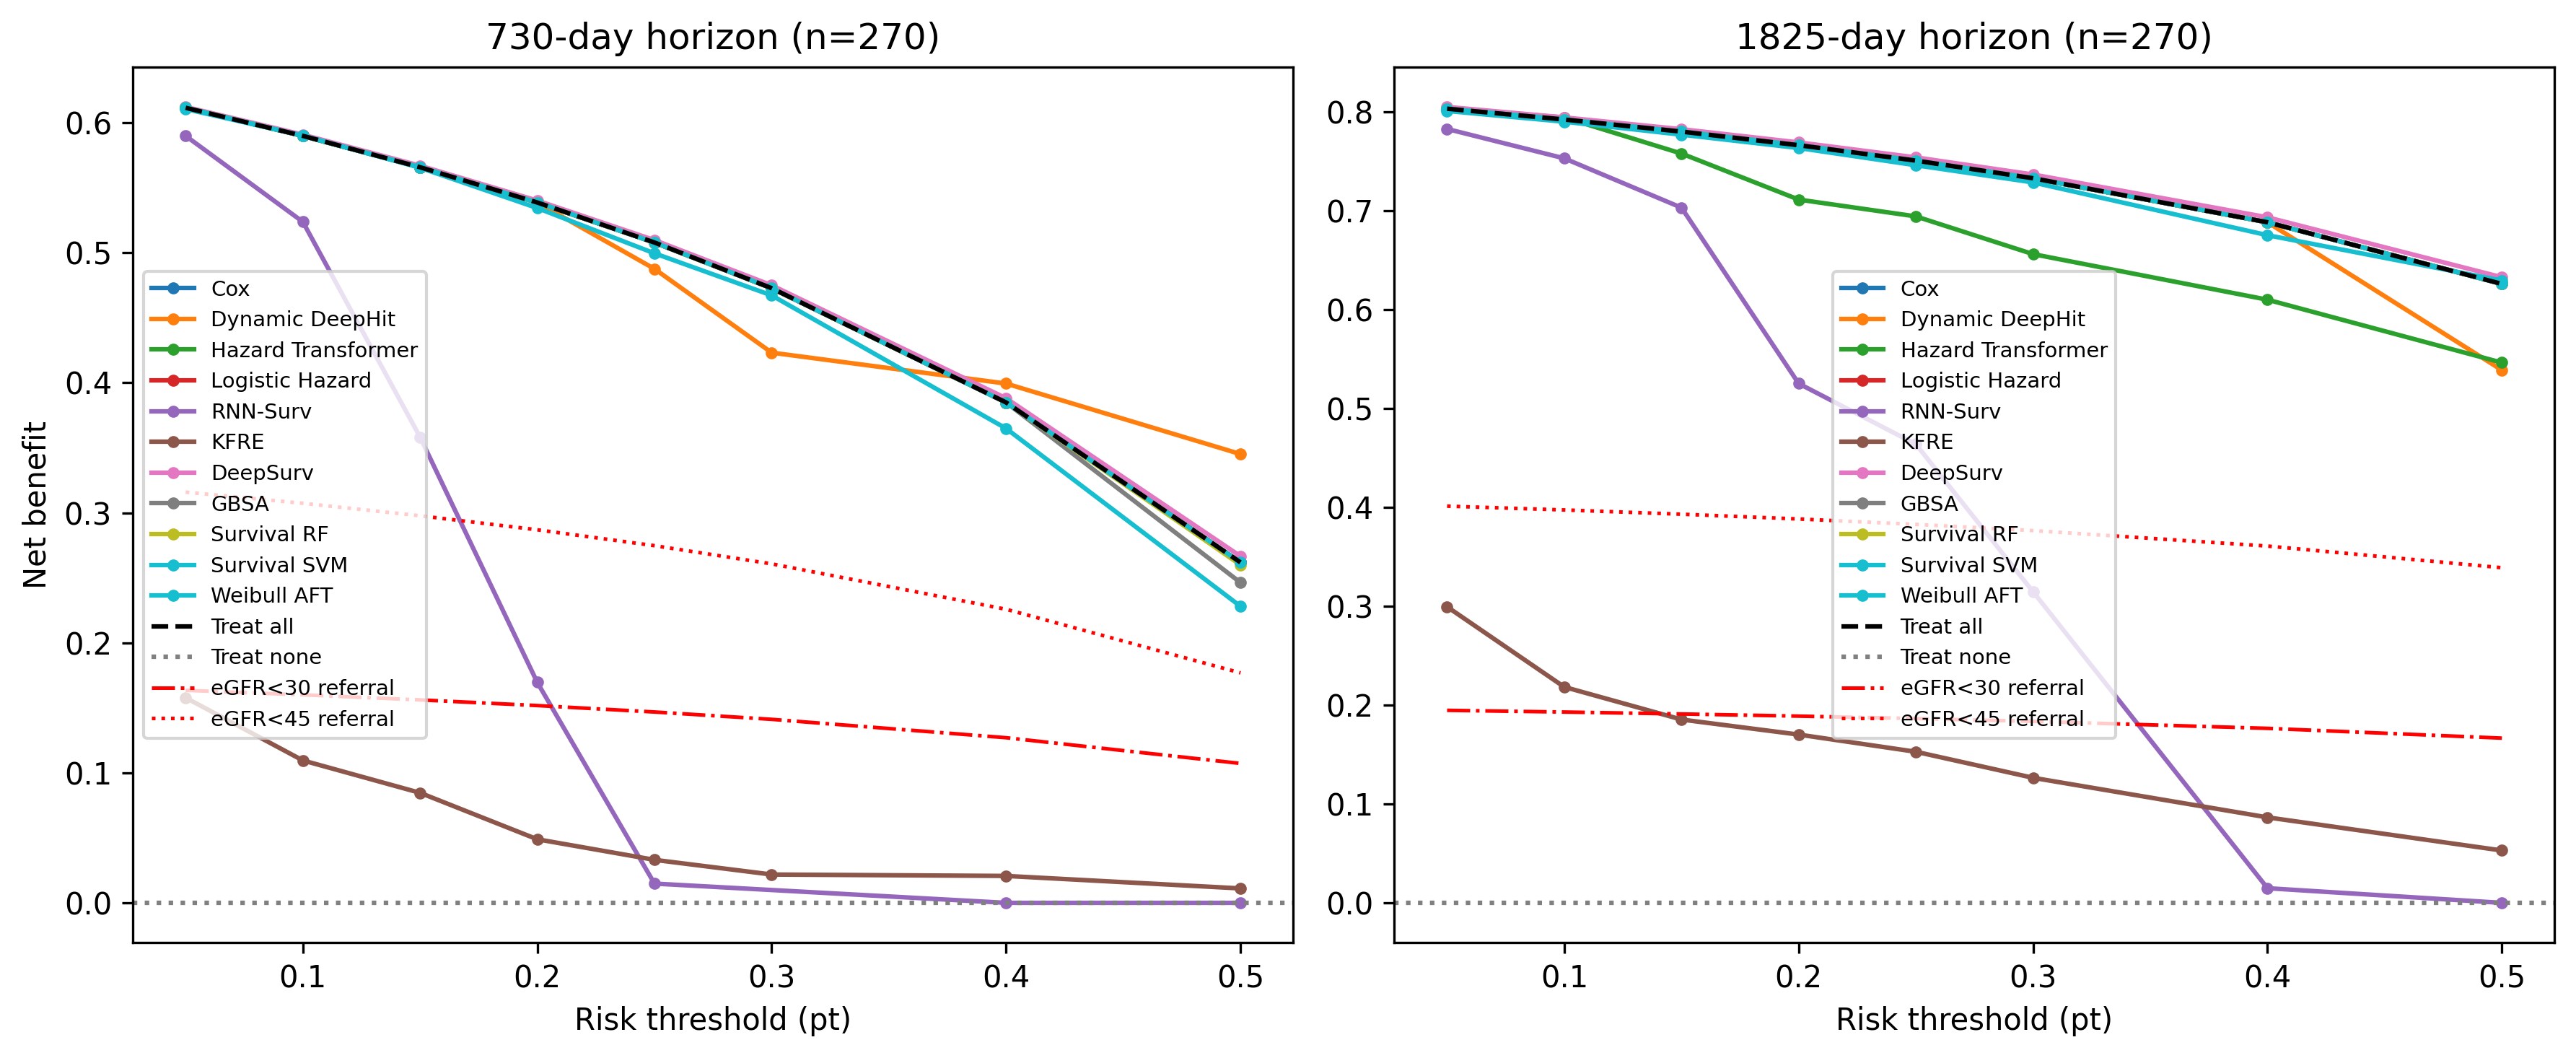
\includegraphics[width=\textwidth]{figs/four_features_decision_curve_plot.png}
    \caption{{\bf Four-feature holdout decision curves at 2 and 5 years (repetition 1).} Net benefit across risk thresholds for each model, treat-all, treat-none, and eGFR $<$30 and $<$45 referral rules, all evaluated on the same holdout patients and patient-level outcomes.}
    \label{fig:dca_four}
\end{figure}

\textbf{Treat-all is a strong comparator in these cohorts.} Because most patients reach the labelled event, treating everyone has high net benefit: at two years, averaged over the five repetitions, 0.615 at a 0.05 threshold falling to 0.269 at 0.50 with four features, and 0.787 to 0.596 with eight features (Fig.~\ref{fig:dca_four}). Most learned models assign above-threshold risk to nearly every patient and so match treat-all without exceeding it. The eGFR referral rules (four-feature two-year net benefit 0.187--0.110 for eGFR $<$30 and 0.346--0.183 for $<$45) and KFRE (0.166--0.017) fall well below treat-all at every threshold; KFRE's low net benefit follows from the underprediction above, since few patients exceed the thresholds.

\textbf{Only Dynamic-DeepHit adds net benefit over treat-all, and only at higher thresholds.} With four features at two years, Dynamic-DeepHit matches treat-all up to a 0.30 threshold and exceeds it at 0.40 (0.430 versus 0.391) and 0.50 (0.390 versus 0.269). With eight features its advantage at those thresholds is small (0.672 versus 0.663 and 0.608 versus 0.596). In the twenty-feature cohort it exceeds treat-all at thresholds of 0.20 and above, increasingly so as the threshold rises (0.640 versus 0.613 at 0.25; 0.558 versus 0.428 at 0.50). At five years, no model consistently exceeds treat-all. Eight- and twenty-feature decision curves are in Supplementary Fig.~S4 and Supplementary Fig.~S5. These are thresholds at which a clinician would refer only patients with substantial predicted risk; whether such thresholds match referral practice is outside the scope of this retrospective analysis.

\subsection{Subgroup performance}

\begin{table}[h!]
\centering
\footnotesize
\setlength{\tabcolsep}{3pt}
\begin{tabular}{@{}lcccccc@{}}
\toprule
 & \multicolumn{2}{c}{\textbf{Four features}} & \multicolumn{2}{c}{\textbf{Eight features}} & \multicolumn{2}{c}{\textbf{Twenty features}} \\
\cmidrule(lr){2-3}\cmidrule(lr){4-5}\cmidrule(lr){6-7}
\textbf{Group} & \textbf{DDH} & \textbf{KFRE} & \textbf{DDH} & \textbf{KFRE} & \textbf{DDH} & \textbf{HT} \\
\midrule
Age 18--45 & 0.869$^{4}$ & 0.557$^{4}$ & -- & -- & 0.871 & 0.742 \\
Age 46--65 & 0.844 & 0.474 & 0.842 & 0.511 & 0.836 & 0.756 \\
Age 66--85 & 0.854 & 0.606 & 0.806 & 0.560 & 0.880 & 0.761 \\
Age $>$85 & -- & -- & -- & -- & 0.894 & 0.782 \\
Female & 0.844 & 0.537 & 0.816 & 0.496 & 0.885 & 0.769 \\
Male & 0.858 & 0.549 & 0.834 & 0.539 & 0.868 & 0.756 \\
White & 0.857 & 0.574 & 0.839 & 0.536 & 0.864 & 0.758 \\
Black & 0.845 & 0.495 & 0.824$^{4}$ & 0.497$^{4}$ & 0.841 & 0.755 \\
Hispanic/Latino & 0.867$^{3}$ & 0.479$^{3}$ & -- & -- & 0.870 & 0.769 \\
Asian & -- & -- & -- & -- & 0.843 & 0.733 \\
Other & -- & -- & -- & -- & 0.895 & 0.766 \\
Unknown/not recorded & -- & -- & -- & -- & 0.800 & 0.720 \\
\bottomrule
\end{tabular}
\caption{{\bf Holdout C-index within demographic groups.} Mean across the repetitions in which the group met the minimum size (at least 20 patients and 5 events in the holdout); a superscript gives the number of repetitions when fewer than five, and ``--'' marks groups that never met it. DDH, Dynamic-DeepHit; HT, Hazard Transformer. Age is MIMIC-IV \texttt{anchor\_age}, not age at the prediction landmark. All models, IBS, AUC, and per-repetition intervals are in Supplementary Table~S1.}
\label{tab:subgroup}
\end{table}

Table~\ref{tab:subgroup} reports the C-index within age, sex, and race groups for the best model in each scenario and for KFRE. Dynamic-DeepHit's C-index lies between 0.84 and 0.87 in every evaluable four-feature group, between 0.81 and 0.84 in every eight-feature group, and between 0.80 and 0.90 in every twenty-feature group, with its lowest value in patients whose race was not recorded. KFRE's C-index varies more across groups, from 0.474 (age 46--65) to 0.606 (age 66--85) with four features, and is lower in Black (0.495) and Hispanic/Latino (0.479) than in White patients (0.574). Small groups limit these comparisons: in the four-feature holdout, patients over 85, Asian patients, and patients of other recorded races never reached the minimum size, and several groups have about 25--70 patients, so within-group intervals are wide (Supplementary Table~S1). These numbers describe performance within groups and do not establish fairness.

\subsection{Feature importance}

Fig.~\ref{fig:feature_importance_four} shows the four-feature importance diagnostics for repetition 1, with the eight-feature companion in Supplementary Fig.~S1.

\begin{figure}[h!]
    \centering
    
\includegraphics[width=\textwidth]{figs/four_features_all_models_feature_importance.png}
    \caption{{\bf Four-feature importance diagnostics (repetition 1).} Each panel uses that model's own importance measure (coefficients, native or permutation importance, or input gradients); scales are not comparable across panels. These are not SHAP values.}
    \label{fig:feature_importance_four}
\end{figure}

Rankings differ by model and measure. GBSA ranks eGFR (0.394) and uACR (0.377) highest, Survival RF's permutation importance ranks eGFR highest (0.031), and RNN-Surv's gradients are largest for eGFR (0.290). Dynamic-DeepHit's and DeepSurv's gradients are largest for sex (0.301 and 0.280), and Hazard Transformer's and Logistic Hazard's for age (0.331 and 0.325). The raw-scale coefficients of Cox, Weibull AFT, and Survival SVM are small and scale-dependent; a uACR coefficient near zero reflects its large numeric range rather than its exclusion. These within-model summaries do not establish a common biological ranking. In the twenty-feature cohort, the gradient calculations for Dynamic-DeepHit and Hazard Transformer exceeded available memory, so their importance outputs are not interpreted.

% GENERATED from plos_digital_health.tex by scripts/plos_to_sections.py -- edit the PLOS
% file and rerun the script rather than editing this file directly.

\section{Discussion}

\textbf{A history-aware model separates from the rest; most others match KFRE.} On holdout patients that no model saw during development, Dynamic-DeepHit had the highest discrimination in all three scenarios, and its advantage over KFRE excluded zero in every repetition. Hazard Transformer, the other model that reads patient histories, was second in the twenty-feature cohort. Most other learned models, which score a single final observation, were not distinguishable from KFRE in ranking patients. These results describe the implemented models under this evaluation protocol; they do not establish the intrinsic superiority of an architecture.

\textbf{Feature count is confounded with cohort and with access to history.} The eight-feature complete-case cohort is smaller and has shorter follow-up than the four-feature cohort, and the twenty-feature representation includes missingness indicators and a much broader patient group. Dynamic-DeepHit and Hazard Transformer use patient histories, whereas most comparators use final observations. Both population selection and access to longitudinal information can affect performance, and their contributions cannot be separated here. A matched-patient, matched-history ablation is needed to isolate the contribution of additional measurements or architecture.

\textbf{Ranking, calibration, and net benefit tell different stories.} KFRE ranks patients about as well as most learned models but underestimates absolute risk severely in this cohort, which drives both its high Brier scores and its low net benefit. Hazard Transformer ranks twenty-feature patients well yet assigns the same two-year risk to everyone. Because most patients in these cohorts reach the labelled event, treat-all is a demanding comparator, and only Dynamic-DeepHit exceeded it, at higher thresholds. Any clinical use would require recalibration to the target population and outcome and a decision threshold justified by referral practice.

\textbf{Discrimination was similar across demographic groups for the best model.} Dynamic-DeepHit's C-index varied little across age, sex, and recorded race groups in all three scenarios, whereas KFRE's varied more. This is reassuring only within the limits of the group sizes and of anchor-year age and administratively recorded race; it is not a fairness assessment.

\subsection{Limitations} \label{sec:limitations}

\begin{itemize}
    \item \textbf{Single data source; internal validation only.} All patients come from one academic medical centre. The holdout is a random patient-level split of the same cohort, so it measures performance on new patients from the same population, not transportability to other hospitals, periods, or primary-care settings. The selected hospital cohort is event-rich and differs from the populations supporting KFRE's published validation; performance here should not be generalized to routine clinical screening.
    \item \textbf{The labelled outcome is not the KFRE endpoint.} The event is an acute or unspecified kidney-failure diagnosis code recorded in a patient with CKD stage 3--5, dated to the admission that carried it, not the initiation of maintenance dialysis or preemptive transplantation that KFRE predicts (Section~\ref{sec:outcome}). Reported calibration differences between KFRE and the fitted models therefore combine an endpoint difference, a population difference, and the fitted/externally-specified asymmetry, and this benchmark does not separate them.
    \item \textbf{Time origin and follow-up.} Durations are measured from each patient's first extracted laboratory record, not from a common prospective landmark, and follow-up before the labelled event is short in the complete-case cohorts (median 16 days with four features and 0.4 days with eight among label-positive patients; 23--31\% of patients contribute one row). A two-year horizon from that origin is a follow-up window, not a prediction lead time, and final-observation scoring for some models and full-history scoring for others is not a common landmark design.
    \item \textbf{Degenerate predictions.} Hazard Transformer produces constant two-year probabilities, and Cox is below chance in the twenty-feature cohort (C-index 0.473). These behaviors repeat across repetitions, and no causal explanation is established here.
    \item \textbf{No competing-risk assessment.} Death before ESRD is not modeled as a competing event, which can inflate predicted risks for patients at high risk of death.
    \item \textbf{Uncertainty and subgroups.} Bootstrap intervals hold the fitted models and the censoring reference fixed, and paired comparisons are not adjusted for multiplicity. Subgroup analyses use anchor-year age and administratively recorded race, several groups are small, and some never reach the minimum size.
    \item \textbf{Importance diagnostics are heterogeneous and partly incomplete.} Coefficients, gradients, and permutation scores have different meanings and scales, and the twenty-feature gradient analyses for Dynamic-DeepHit and Hazard Transformer failed for lack of memory.
\end{itemize}

\subsection{Future work}
External validation in other health systems, with dialysis or transplant initiation as the outcome, would test whether the advantage of history-aware models transfers and allow a like-for-like comparison with KFRE. A common prospective landmark with an explicit information cutoff, explicit competing-risk modelling, recalibration to the target population, matched-cohort feature ablations, and memory-bounded feature-importance calculations would address the remaining gaps.


\backmatter

\section*{Declarations}
\begin{itemize}
\item Funding: Not applicable.
\item Conflict of interest: The authors declare no competing interests.
\item Ethics approval and consent to participate: Secondary analysis of de-identified MIMIC-IV v2.2 data. The Beth Israel Deaconess Medical Center institutional review board approved the MIMIC-IV data-sharing initiative and waived informed consent; data were accessed through PhysioNet credentialed access (Section~\ref{sec:ethics}).
% AUTHOR TO CONFIRM BEFORE SUBMISSION: add the authors' own institutional determination for this analysis.
\item Data availability: MIMIC-IV v2.2 is available from PhysioNet (\url{https://doi.org/10.13026/6mm1-ek67}) to credentialed users who complete the required training and sign the data use agreement; the authors cannot redistribute it. The cohort-extraction code reproduces the analysis cohorts.
\item Code availability: Benchmark code, extraction pipeline, and analysis scripts are available in the project repository.
\item Reporting: This study follows TRIPOD+AI; the completed checklist is provided as Supplementary Information.
\item Author contribution: All authors contributed to study design, experimentation, analysis, and manuscript preparation.
\end{itemize}

\bibliography{sn-bibliography}

\end{document}
